\documentclass{article}
\usepackage{mathtools}
\usepackage{color}
\usepackage[utf8]{inputenc}
\usepackage{mathtools}
\usepackage{graphicx}
\usepackage{placeins}
\graphicspath{ {./img/} }
\begin{document}
\title{TDT4136 - Assignment 5}
\author{Filip F Egge}
\date{October 3, 2014}
\maketitle

\newpage
\section*{Solving Contraint Satisfaction Problems}
\subsection*{Solved boards}
	\FloatBarrier
	\begin{figure}[!htb]
		\caption{Easy}
		\centering
		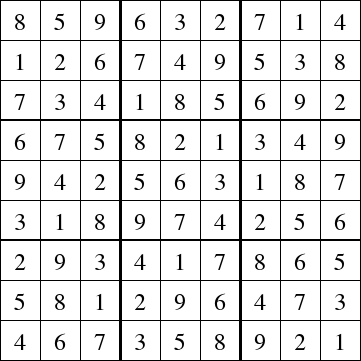
\includegraphics[width=0.5\textwidth]{easy.png}
	\end{figure}

	\begin{figure}[!htb]
		\caption{Medium 1-2}
		\centering
		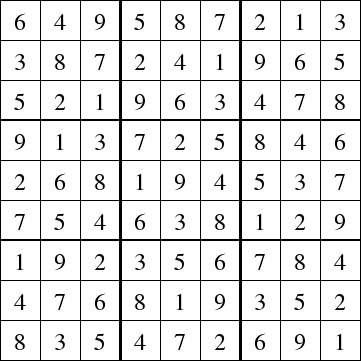
\includegraphics[width=0.5\textwidth]{medium.png}
	\end{figure}
	\begin{figure}[!htb]
		\caption{Hard 1-3}
		\centering
		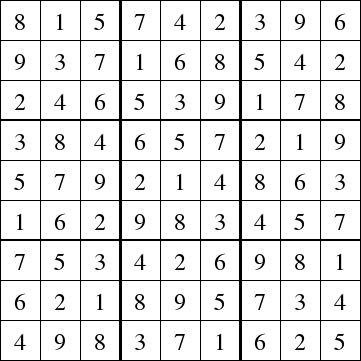
\includegraphics[width=0.5\textwidth]{hard.png}
	\end{figure}
	\begin{figure}[!htb]
		\caption{Very hard 1-4}
		\centering
		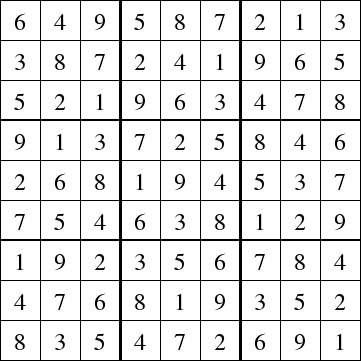
\includegraphics[width=0.5\textwidth]{medium.png}
	\end{figure}
\FloatBarrier
\subsection*{Something}
	Something
\end{document}